\documentclass{beamer}


% Packages
\usepackage{graphicx}
\usepackage{hyperref}
\usepackage{moreverb}
\usepackage{tikz}
\usepackage{xcolor}

% Theme
\usecolortheme{whale}

% Color definitions
\definecolor{solarOrange}{HTML}{E98300}
\definecolor{spaceBlue}{HTML}{0039A6}
\definecolor{callierGray}{HTML}{766A62}
\definecolor{sparkOrange}{HTML}{FFB612}
\definecolor{stratosBlue}{HTML}{00A1DE}
\definecolor{skyBlue}{HTML}{5BC6EB}
\definecolor{ecoGreen}{HTML}{008542}
\definecolor{saplingGreen}{HTML}{69BE28}
\definecolor{seedlingGreen}{HTML}{C9DD03}


\renewcommand{\listinglabel}[1]{\llap{\tiny\sffamily\the#1}\hskip\listingoffset\relax}


\title{\texttt{callierr}: Visually Communicate Data in R using the Callier Center's Color Palette}
\author{Patrick Reidy}
\date{January 20, 2017}
\institute{Callier Center for Communication Disorders}




\begin{document}
\frame{\titlepage}


\begin{frame}
\frametitle{R graphics ecosystem}
\begin{description}
 \item [R] a freely available language and environment for statistical computing and graphics 
   \newline{}{\footnotesize (\url{https://cran.r-project.org})}
 \item [graphics] the pre-installed base plotting system for R
 \item [ggplot2] a plotting system for R based on the Grammar of Graphics 
   \newline{}{\footnotesize (\url{http://ggplot2.org})}
 \item [callierr] an R package that provides color palettes and scales based on the Callier Center Brand Standards; integrates with \texttt{graphics} and \texttt{ggplot2}
   \newline{}{\footnotesize (\url{https://github.com/patrickreidy/callierr})}
\end{description}
\end{frame}



\begin{frame}[t]
 \frametitle{Callier Center color palette}
 \begin{center}
  \only<1>{
   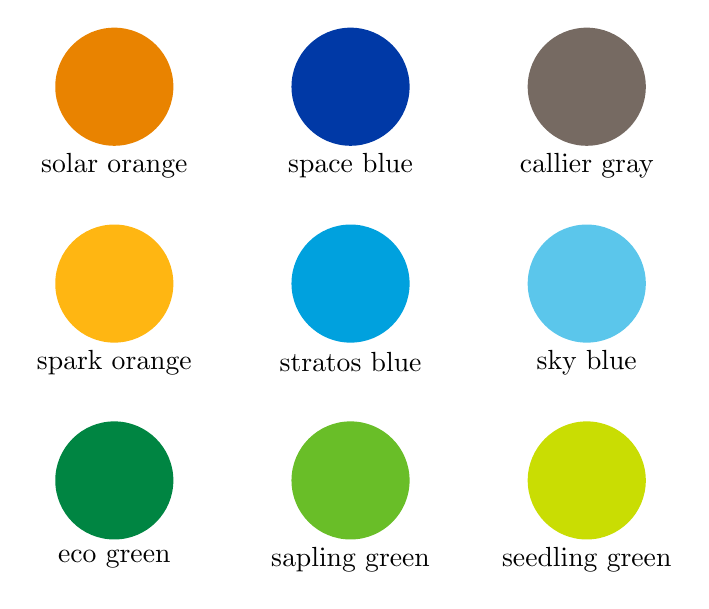
\begin{tikzpicture}
     % Primary colors.
     \fill [fill=solarOrange] (0,0) circle [radius=0.75cm];
      \node at (0,-1) {solar orange};
     \fill [fill=spaceBlue] (3,0) circle [radius=0.75cm];
      \node at (3, -1) {space blue};
     \fill [fill=callierGray] (6,0) circle [radius=0.75cm];
      \node at (6, -1) {callier gray};
     % Secondary colors.
     \fill [fill=sparkOrange] (0,-2.5) circle [radius=0.75cm];
      \node at (0,-3.5) {spark orange};
     \fill [fill=stratosBlue] (3,-2.5) circle [radius=0.75cm];
      \node at (3,-3.5) {stratos blue};
     \fill [fill=skyBlue] (6,-2.5) circle [radius=0.75cm];
      \node at (6,-3.5) {sky blue};
     % Tertiary colors.
     \fill [fill=ecoGreen] (0, -5) circle [radius=0.75cm];
      \node at (0,-6) {eco green};
     \fill [fill=saplingGreen] (3, -5) circle [radius=0.75cm];
      \node at (3,-6) {sapling green};
     \fill [fill=seedlingGreen] (6, -5) circle [radius=0.75cm];
      \node at (6,-6) {seedling green};
   \end{tikzpicture}
  }
  \only<2>{
   \vspace{1em}
   \includegraphics[width=0.95\textwidth]{tina-noncanonical}
  }
 \end{center}
\end{frame}



\begin{frame}[fragile]
\frametitle{\texttt{callierr}: Object hierarchy}
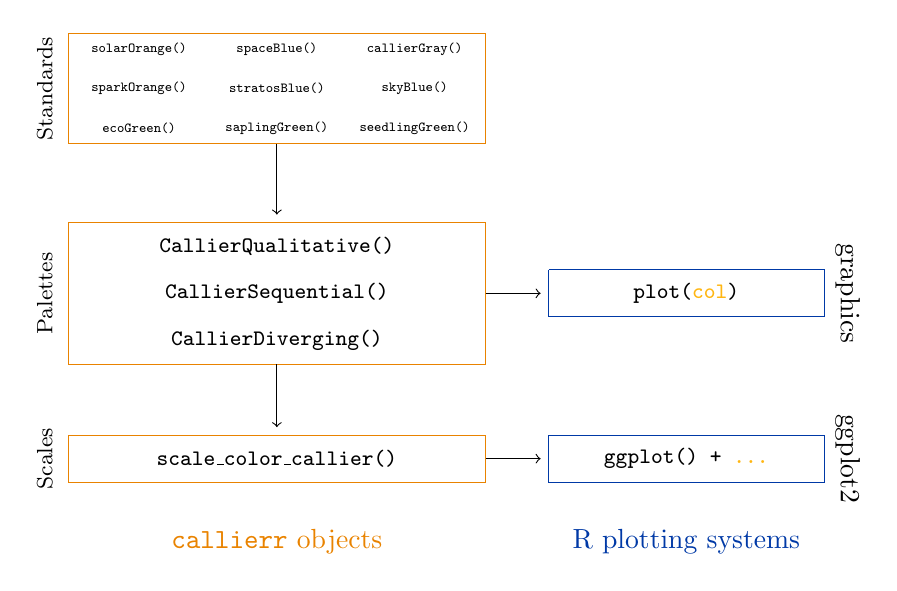
\begin{tikzpicture}
 % Constants
 \node[rotate=90] at (-1.2,-0.5) {\footnotesize Standards};
 \draw[draw=solarOrange] (-0.9,0.2) -- (4.4,0.2) -- (4.4,-1.2) -- (-0.9,-1.2) -- (-0.9,0.2);
 \node at (0,0) {\tiny \texttt{solarOrange()}};
 \node at (1.75,0) {\tiny \texttt{spaceBlue()}};
 \node at (3.5,0) {\tiny \texttt{callierGray()}};
 \node at (0,-0.5) {\tiny \texttt{sparkOrange()}};
 \node at (1.75,-0.5) {\tiny \texttt{stratosBlue()}};
 \node at (3.5,-0.5) {\tiny \texttt{skyBlue()}};
 \node at (0,-1) {\tiny \texttt{ecoGreen()}};
 \node at (1.75,-1) {\tiny \texttt{saplingGreen()}};
 \node at (3.5,-1) {\tiny \texttt{seedlingGreen()}};
 \draw [->] (1.75,-1.2) -- (1.75,-2.1);
 % Palettes
 \node[rotate=90] at (-1.2,-3.1) {\footnotesize Palettes};
 \draw[draw=solarOrange] (-0.9,-2.2) -- (4.4,-2.2) -- (4.4,-4) -- (-0.9,-4) -- (-0.9,-2.2);
 \node at (1.75,-2.5) {\footnotesize \texttt{CallierQualitative()}};
 \node at (1.75,-3.1) {\footnotesize \texttt{CallierSequential()}};
 \node at (1.75,-3.7) {\footnotesize \texttt{CallierDiverging()}};
 \draw [->] (1.75,-4) -- (1.75,-4.8);
 \draw [->] (4.4,-3.1) -- (5.1,-3.1);
 % Scales
 \node[rotate=90] at (-1.2,-5.2) {\footnotesize Scales};
 \draw[draw=solarOrange] (-0.9,-4.9) -- (4.4,-4.9) -- (4.4,-5.5) -- (-0.9,-5.5) -- (-0.9,-4.9);
 \node at (1.75,-5.2) {\footnotesize \texttt{scale\_color\_callier()}};
 \draw [->] (4.4,-5.2) -- (5.1,-5.2);
 % Palette output
 \node[rotate=270] at (9,-3.1) {graphics};
 \draw[draw=spaceBlue] (5.2,-2.8) -- (8.7,-2.8) -- (8.7,-3.4) -- (5.2,-3.4) -- (5.2,-2.8);
 \node at (6.95,-3.1) {\footnotesize \texttt{plot(\color{sparkOrange}{col}\color{black})}};
 % Scale output
 \node[rotate=270] at (9,-5.2) {ggplot2};
 \draw[draw=spaceBlue] (5.2,-4.9) -- (8.7,-4.9) -- (8.7,-5.5) -- (5.2,-5.5) -- (5.2,-4.9);
 \node at (6.95,-5.2) {\footnotesize \texttt{ggplot() + \color{sparkOrange}{...}}};
 % Rug labels
 \node at (1.75,-6.25) {\color{solarOrange}{\texttt{callierr} objects}};
 \node at (6.95,-6.25) {\color{spaceBlue}{R plotting systems}};
\end{tikzpicture} 
\end{frame}



\begin{frame}[fragile,t]
\frametitle{\texttt{ggplot()}'s default colors}
\begin{listing}{1}
base_plot <- 
  ggplot(data=diamonds,
         aes(x=carat, y=price, color=color)) +
  geom_smooth()
\end{listing}
\begin{tikzpicture}[remember picture,overlay]
    \node[yshift=2.75cm] at (current page.south) {\includegraphics{flash-diamonds-base}};
\end{tikzpicture}
\end{frame}


\begin{frame}
\frametitle{\texttt{callierr} in action: Qualitative scheme}
\begin{center}
\begin{tikzpicture}
 \draw (1*360/7: 3cm) node{G};
 \draw (2*360/7: 3cm) node{D};
 \draw (3*360/7: 3cm) node{J};
 \draw (4*360/7: 3cm) node{E};
 \draw (5*360/7: 3cm) node{H};
 \draw (6*360/7: 3cm) node{I};
 \draw (7*360/7: 3cm) node{F};
 \draw (0*360/7: 0cm) node{{\Huge ?}};
\end{tikzpicture}
\end{center}
\end{frame}

\begin{frame}[fragile,t]
\frametitle{\texttt{callierr} in action: Qualitative scheme}
\begin{listing}{1}
base_plot +
  scale_color_callier(
    scheme = "qualitative", steps = 7)
\end{listing}
\begin{tikzpicture}[remember picture,overlay]
    \node[yshift=2.75cm] at (current page.south) {\includegraphics{flash-diamonds-qual}};
\end{tikzpicture}
\end{frame}



\begin{frame}
\frametitle{\texttt{callierr} in action: Sequential scheme}
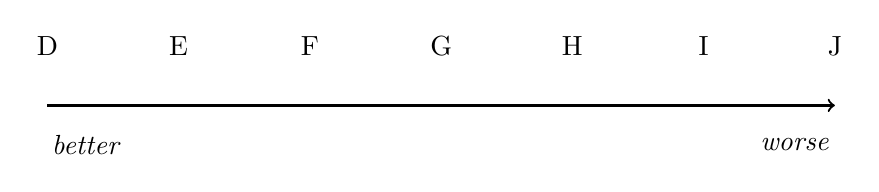
\begin{tikzpicture}
 \node at (0,0) {D};
 \node at (1.666,0) {E};
 \node at (3.333,0) {F};
 \node at (5,0) {G};
 \node at (6.666,0) {H};
 \node at (8.333,0) {I};
 \node at (10,0) {J};
 \draw [->,thick] (0,-0.75) -- (10,-0.75);
 \node[align=left] at (0.5,-1.25) {\textit{better}};
 \node[align=right] at (9.5, -1.25) {\textit{worse}};
\end{tikzpicture}

\vspace{2em}

\begin{itemize}
 \item Differences between levels $=$ differences in luminosity
\end{itemize}
\end{frame}

\begin{frame}[fragile,t]
\frametitle{\texttt{callierr} in action: Sequential scheme}
\begin{listing}{1}
base_plot +
  scale_color_callier(
    scheme = "sequential", steps = 7, 
    hue = "orange", direction = "decreasing")
\end{listing}
\begin{tikzpicture}[remember picture,overlay]
    \node[yshift=2.75cm] at (current page.south) {\includegraphics{flash-diamonds-seq}};
\end{tikzpicture}
\end{frame}



\begin{frame}
\frametitle{\texttt{callierr} in action: Diverging scheme}
\begin{tikzpicture}
 \node at (0,0) {D};
 \node at (1.666,0) {E};
 \node at (3.333,0) {F};
 \node at (5,0) {G};
 \node at (6.666,0) {H};
 \node at (8.333,0) {I};
 \node at (10,0) {J};
 \draw (0,0.25) -- (0,0.75) -- (3.333,0.75) -- (3.333,0.25);
 \node at (1.666,1) {\textit{colorless}};
 \draw (5,-0.25) -- (5,-0.75) -- (10,-0.75) -- (10,-0.25);
 \node at (7.5,-1) {\textit{near colorless}};
\end{tikzpicture}

\vspace{2em}

\begin{itemize}
 \item Differences within a group $=$ differences in luminosity
 \item Differences between groups $=$ differences in hue
\end{itemize}
\end{frame}

\begin{frame}[fragile,t]
\frametitle{\texttt{callierr} in action: Diverging scheme}
\begin{listing}{1}
base_plot +
  scale_color_callier(
    scheme = "diverging",
    steps = list(orange = c("D", "E", "F"),
                 blue = c("G", "H", "I", "J")))
\end{listing}
\begin{tikzpicture}[remember picture,overlay]
    \node[yshift=2.75cm] at (current page.south) {\includegraphics{flash-diamonds-div}};
\end{tikzpicture}
\end{frame}



\begin{frame}[fragile]
\frametitle{\texttt{ColorChart()}: Dichromats are people too}
\begin{listing}{1}
s <- list(orange = c("D", "E", "F"), 
          blue = c("G", "H", "I", "J"))
p <- CallierDiverging(steps = s)
ColorChart(palette = p)
\end{listing}

\hspace{-0.7cm}
\includegraphics{flash-color-chart}
\end{frame}



\begin{frame}
\frametitle{Source directory organization for R packages}
\begin{description}
 \item [{\scriptsize DESCRIPTION}] Metadata
 \item [{\scriptsize NAMESPACE}] Export and import statements
 \item [R/] Code files (.R extension) where objects are defined
 \item [man/] Documentation files for the exported objects
\end{description}
\end{frame}



\begin{frame}
\frametitle{Final thoughts}
\begin{itemize}
 \item Focus on the structure within data that you want to communicate 
 
 Let \texttt{callierr} map that structure into a color scheme
 \vspace{1em}
 \item \texttt{callierr}'s code is open source; its license is copyleft
 \begin{itemize}
  \item Contribute new functionality through Github
  \item Adapt to other programming languages
 \end{itemize}
 \vspace{1em}
 \item Future developments:
 \begin{itemize}
  \item \texttt{ColorChart()}: accept scales, not just palettes
  \item Diverging schemes: generalize beyond 1-d schemes
 \end{itemize}
\end{itemize}
\end{frame}


\end{document}


